\documentclass[10pt,twocolumn]{article}
\usepackage[letterpaper,top=0.64in,bottom=0.68in,left=0.66in,right=0.66in,columnsep=0.24in]{geometry}
\usepackage[T1]{fontenc}\usepackage{lmodern}\usepackage{microtype}\usepackage{graphicx}\usepackage{booktabs}
\usepackage{array}\usepackage{caption}\usepackage{xcolor}\usepackage{enumitem}\usepackage{tikz}
\usepackage{balance}
\usetikzlibrary{positioning}
\usepackage[hidelinks]{hyperref}\usepackage{url}
\definecolor{sprited}{HTML}{6337C7}\definecolor{teal}{HTML}{008C95}\definecolor{pale}{HTML}{F3F0FA}\definecolor{muted}{HTML}{555555}
\hypersetup{colorlinks=true,linkcolor=sprited,citecolor=sprited,urlcolor=sprited,
pdftitle={Dancing Stick Figures: A Synthetic Video Dataset, Renderer, and Diagnostic Evaluation Suite},
pdfauthor={Jin Hyuk Cho},pdfsubject={Synthetic video dataset, renderer, and diagnostic evaluation suite},
pdfkeywords={video generation, benchmark, synthetic dataset, structural evaluation, education}}
\captionsetup{font=small,labelfont=bf,skip=4pt}\setlist{nosep,leftmargin=*}
\setlength{\parindent}{1em}\setlength{\parskip}{0pt}\setlength{\textfloatsep}{8pt plus 2pt minus 2pt}
\setlength{\floatsep}{7pt plus 2pt minus 2pt}\setlength{\intextsep}{7pt plus 2pt minus 2pt}\renewcommand{\arraystretch}{1.08}

\title{\vspace{-1.5em}\textbf{Dancing Stick Figures: A Synthetic Video Dataset,\\Renderer, and Diagnostic Evaluation Suite}}
\author{Jin Hyuk Cho\\Sprited\\\small\href{mailto:jin@sprited.ai}{jin@sprited.ai} $\cdot$
\href{https://orcid.org/0009-0001-1896-8242}{ORCID 0009-0001-1896-8242}\\[-2pt]
\small\href{https://huggingface.co/datasets/sprited/dancing-stick-figures}{Dataset} $\cdot$
\href{https://github.com/sprited-ai/dancing-stick-figures}{Code} $\cdot$
\href{https://huggingface.co/sprited/dancing-stick-figures-baselines}{Models} $\cdot$
\href{https://colab.research.google.com/github/sprited-ai/dancing-stick-figures/blob/main/notebooks/dancing_stick_figures_colab_v0_3.ipynb}{Colab}}
\date{}

\begin{document}\raggedbottom\maketitle\vspace{-1.25em}
\begin{abstract}
Video generation is difficult to learn by doing. Real video datasets are large, the process that produced each
frame is unknown, and a single quality score rarely identifies why a generated video failed. We introduce
\textbf{Dancing Stick Figures}, a synthetic video dataset with a deterministic rendering pipeline designed for end-to-end
experiments on one conventional GPU. It contains 1,340 six-second motions rendered from three cameras, for 4,020 videos
and 482,400 labelled frames. Every frame remains linked to the joints, camera, body parameters, depth, surface normals,
body-part labels, and source motion that produced it. This known state acts as an answer key for evaluation. We provide
measurements of whether coloured limbs remain connected, whether the figure remains intact, and how its position and
pose change over time. Controlled mistakes test which failures each measurement can and cannot detect. In a controlled
120-frame study, reversal leaves the reported time-symmetric motion signals unchanged and produces essentially the
same FVD as the untouched real reference. The release includes a 0.85-GB $64^2$ configuration, an optional
$32^2$ route, fixed data lists, evaluation scripts, checkpoints, and a Colab lesson that trains an image generator
and then a video generator. Together, these components provide an accessible route for observing how video generation
works and why it fails: a small, complete first experiment in video generation.
\end{abstract}

\section{Introduction}
Video generation is easy to encounter and hard to study. Frontier systems such as Seedance and MiniMax
H3~\cite{gao2025seedance,minimax2026h3} make compelling generated videos visible through products, technical reports,
and released artifacts. For a learner, however, access to results---or even to weights---does not resolve three
barriers:
\begin{itemize}[leftmargin=*,nosep]
\item \textbf{Data and reproduction.} Open weights permit inference and adaptation, but without the training dataset a
reader cannot reconstruct the learning problem, reproduce the run, or trace a failure back to the data. Public video
datasets exist, yet the exact data, filters, annotations, model, and data-to-model recipe behind a frontier system are
rarely released as one reproducible whole.
\item \textbf{Experimentation.} Frontier training typically requires large-scale video datasets, substantial compute,
and pretrained compression and conditioning systems. The available learning path is consequently skewed toward
prompting and fine-tuning pretrained artifacts. Reading the backbone, adding a conditioning input, and retraining a
controlled variant within hours remain difficult.
\item \textbf{Evaluation and explanation.} ``Better generation'' may mean cleaner frames, stronger prompt adherence,
intact body structure, plausible motion, or temporal consistency; these properties can change separately. An aggregate
score does not say which visible property changed, while a failure may originate in the data, compression,
conditioning, temporal model, rollout context, or sampler.
\end{itemize}

These barriers give three design criteria for a course-scale dataset and reference experiment:
\begin{enumerate}[leftmargin=*,nosep]
\item \textbf{Compute.} The complete image-to-video training path must fit a single consumer GPU or a commonly available Colab runtime;
\item \textbf{Turnaround.} Training must produce inspectable multi-second samples in hours rather than days, leaving time to change the
model and run it again; and
\item \textbf{Diagnosis.} Evaluation must include interpretable measurements of visible structural and temporal failures, together with
controlled tests of what those measurements miss.
\end{enumerate}

The underlying question is practical: can someone with a single GPU train video generation models from
scratch on a small synthetic dataset and study their behaviour through repeated, controlled experiments?
This requires that structural failures be measurable directly, that design contrasts resolve within small
step budgets, and that a failure be traceable to the component that caused it. The corruption study in
\S\ref{sec:results} also measures what the diagnostics themselves miss.

Pretrained generators and adapter methods are productive tools, but they begin after central choices about data,
representation, and architecture have been made. A complementary teaching system should expose the experiment cycle
itself: change one thing, train on a single conventional GPU, inspect the samples, measure the change, and explain the
failure. A small model keeps that complete path---from input data to generated video---within reach of direct study.

Teaching from-scratch video generation requires a complete experiment small enough to repeat. A reader should be able
to download the data, understand what one example contains, train both the spatial and temporal
stages, generate a multi-second result, and diagnose what went wrong. Small datasets reduce cost, but size alone does
not make this loop interpretable: real videos retain unknown camera motion, occlusion, appearance, and annotation
error, while synthetic datasets may provide labels without a route from generation through model training to
evaluation.

Dancing Stick Figures turns that route into a small, complete first experiment. It is first a \emph{dataset and deterministic rendering
pipeline}: a compact collection of articulated motions whose rendered observations remain connected to their exact
generating state. It is also an \emph{evaluation suite}: fixed manifests prevent reference leakage, exact render labels
support failure-specific measurements, and controlled corruptions test whether each measurement responds as intended.
Finally, it includes small pixel-space models that fit this compute envelope. One Colab workflow trains an image
generator, transfers its spatial knowledge to a video generator, trains the video generator itself, samples
multi-second videos, and diagnoses the resulting failures.

The release contributes three implemented pieces:
\begin{enumerate}
\item a label-rich video dataset with a 0.85-GB $64^2$ configuration, optional $32^2$ experiments, the motion,
camera, and body parameters used to render every frame, and a deterministic renderer;
\item a seed-disjoint in-domain evaluation protocol, rule-based structural evaluator, and controlled corruption suite; and
\item runnable image and factorised-DiT video trainers, checkpoints, and an end-to-end Colab curriculum that proceeds
from spatial pretraining to multi-second video generation and diagnosis.
\end{enumerate}

\begin{figure*}[t]\centering
\resizebox{\textwidth}{!}{%
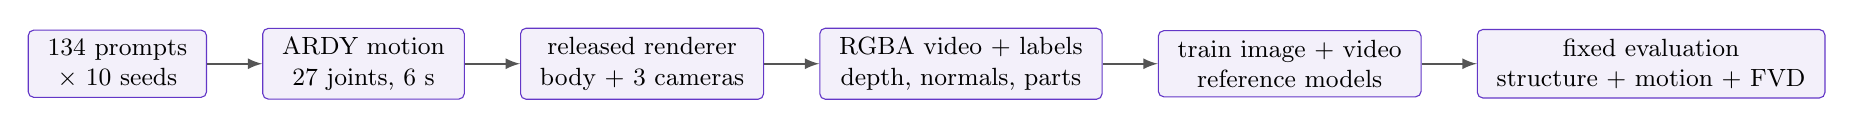
\begin{tikzpicture}[font=\small,node distance=5mm and 7mm,
box/.style={draw=sprited,rounded corners=2pt,fill=pale,align=center,minimum height=8mm,inner xsep=7pt},
arr/.style={-latex,thick,draw=muted}]
\node[box] (prompt) {134 prompts\\$\times$ 10 seeds};
\node[box,right=of prompt] (motion) {ARDY motion\\27 joints, 6 s};
\node[box,right=of motion] (render) {released renderer\\body + 3 cameras};
\node[box,right=of render] (data) {RGBA video + labels\\depth, normals, parts};
\node[box,right=of data] (train) {train image + video\\reference models};
\node[box,right=of train] (eval) {fixed evaluation\\structure + motion + FVD};
\draw[arr] (prompt)--(motion);\draw[arr] (motion)--(render);\draw[arr] (render)--(data);
\draw[arr] (data)--(train);\draw[arr] (train)--(eval);
\end{tikzpicture}}
\caption{The release connects source motions and deterministic rendering to model training and failure-specific evaluation. Every
rendered frame remains linked to the motion, camera, body, and buffers that generated it.}\label{fig:loop}
\end{figure*}

\section{Related Work}
Several research lines provide synthetic video, human-motion supervision, or detailed evaluation. Dancing Stick
Figures combines released data, a renderer, reference models, and measurements in one from-scratch experiment that a
reader can reproduce and alter.

\paragraph{Small and controlled video.} Moving MNIST~\cite{srivastava2015unsupervised} makes temporal prediction cheap
by placing moving digits on a simple canvas, but it offers little articulated structure or language conditioning.
Kubric and MOVi~\cite{greff2022kubric} use a programmable 3D renderer to provide masks, depth, optical flow, and other
ground truth for scene understanding. They show why synthetic control is useful, but neither provides a compact route
from text-conditioned video-generator training to controlled failure diagnosis. We restrict the scene to one
articulated figure so that this entire route remains small enough to rerun and inspect.

\paragraph{Synthetic people.} SURREAL renders more than six million human frames with pose, depth, and part labels
for learning human analysis~\cite{varol2017surreal}. BEDLAM adds realistic bodies, clothing, scenes, and SMPL-X ground
truth, and shows that synthetic-only training can support strong pose-and-shape estimation on real images
~\cite{black2023bedlam}. Both are substantially larger and more realistic human datasets than ours. Their principal
question is whether synthetic people can train perception systems. Ours keeps appearance deliberately simple and asks
whether a reader can train a video generator from scratch, observe its failures, and relate those failures back to the
known motion and rendering state.

\paragraph{Training data for video generation.} Recent datasets address the opacity and quality of frontier training
data directly. HumanVid combines curated real and synthetic data for camera-controllable human animation and identifies
inaccessible training data as an obstacle to transparent comparison~\cite{wang2024humanvid}. MiraData instead targets
long, high-motion videos and detailed structured captions~\cite{ju2024miradata}. These resources optimize coverage,
fidelity, and downstream model capability. They do not aim to make pretraining itself a short experiment or to expose
every factor that produced a frame. Our 0.85-GB tier makes the opposite trade: narrow visual scope in exchange for a
training run and data pipeline that can be inspected together.

Synthetic supervision has also been used to improve capable video generators directly. Zhao et al. mix rendered
video with real data to improve physical fidelity in large pretrained models~\cite{zhao2025synthetic}. DynaVid instead
represents rendered motion as optical flow, then couples a motion generator to a motion-guided video generator for
vigorous human and camera motion~\cite{jin2026dynavid}. These works provide much stronger evidence that synthetic
supervision can improve realistic generation. Our experiment addresses a different computational regime: the reader
can reconstruct the training set and train the reference image and video models without inheriting a large video
generator or a private real-video corpus.

\paragraph{Human motion as source data.} AMASS~\cite{mahmood2019amass} unifies motion-capture collections in a common
body representation, and HumanML3D~\cite{guo2022humanml3d} pairs 3D motion with language. They support motion modelling
without specifying a pixel-video renderer or visual evaluation. We use articulated motion as source material, then
simplify appearance and camera variation so that generated pixels can still be related to joints and limbs. The result
is a diagnostic rendering of motion, not a replacement for realistic human-motion data.

\paragraph{Evaluation of generated video.} FVD~\cite{unterthiner2018fvd} remains useful for distributional comparison,
but controlled studies show that it can respond more strongly to frame content than to temporal corruption
~\cite{ge2024fvdbias}. T2V-CompBench and VBench-2.0 broaden evaluation to prompt composition, human fidelity,
controllability, physics, and commonsense~\cite{sun2025compbench,zheng2025vbench2}. GeneVA localizes human-annotated
spatial and temporal artifacts~\cite{kang2026geneva}, while Ref4D-VideoBench uses reference videos to support
evidence-bounded, instance-level judgments~\cite{wei2026ref4d}. These approaches establish that video quality must be
decomposed rather than reduced to one number. Our contribution is narrower: within one fully specified synthetic domain, controlled
mistakes reveal exactly which structural and motion signals react, which remain unchanged, and what each score cannot
claim. It complements rather than replaces semantic, perceptual, reference-based, or human evaluation.

\section{Dataset and generation pipeline}
Using NVIDIA ARDY~\cite{zhao2026ardy}, we generated one motion at each seed from 0 through 9 for each of 143 prompts
in dance, gesture, locomotion, transition, idle, and sport groups. Each motion is six seconds at 20 fps. A z-buffered capsule renderer with
$4\times$ supersampling emits three deterministic orthographic views. Nine prompts were removed from the release by
visual curation because their motions do not visibly perform the requested action in this rendered domain: near-static
failures (\emph{sways to slow music}), motion the renderer cannot show (\emph{shakes their head no}---the head is a
filled circle), absent or unrecognisable actions (\emph{yoga warrior pose}, \emph{yoga tree pose}, \emph{sit up},
\emph{push up}, and \emph{standing long jump}, whose figure glides forward without an airborne phase), and
interactions with objects that do not exist in the render (\emph{climbs over a low wall}, \emph{lies down on the
floor}). The released collection therefore contains 134 prompts; the exclusion list ships with per-prompt reasons.
Prompts whose stillness is semantically correct (the idle group and stands-\emph{x} prompts) are kept even when the
low-motion QA flag fires. The public data are summarised in
Table~\ref{tab:data}. The split holds prompt vocabulary and camera families fixed while changing the sampled motion:
seeds 0--7 are used for training, seed 8 for validation, and seed 9 for testing. Every prompt therefore appears in
all three splits, but no source-motion realization crosses a split boundary.

\begin{table}[t]\centering\caption{Released data. A motion is rendered from three views.}\label{tab:data}\small
\begin{tabular}{@{}lrrr@{}}\toprule Configuration & Rows & Resolution & Size \\\midrule
\texttt{frames} & 482,400 & $128^2$ & 4.4 GB \\
\texttt{mini} & 482,400 & $64^2$ & 0.79 GB \\
\texttt{motion} & 1,340 & 27 joints & 0.33 GB \\\bottomrule\end{tabular}\end{table}

\begin{table}[t]\centering
\caption{Seed-disjoint in-domain splits. Each split contains all 134 prompts; source motions are disjoint by seed.}
\label{tab:splits}\scriptsize
\begin{tabular}{@{}lrrrr@{}}\toprule
Split & Prompts & Motions & Videos & Frames \\\midrule
Train & 134 & 1,072 & 3,216 & 385,920 \\
Validation & 134 & 134 & 402 & 48,240 \\
Test & 134 & 134 & 402 & 48,240 \\
All & 134 & 1,340 & 4,020 & 482,400 \\\bottomrule
\end{tabular}
\end{table}

\begin{figure*}[t]
\centering

\includegraphics[width=\textwidth]{paper/figs/dataset_anatomy.pdf}
\caption{One released motion viewed through the dataset. (b) Five representative frames selected at equal increments
of pose-space motion, so an idle tail cannot dominate the strip. (a) The middle representative pose from the clip's
three deterministic cameras. (c) The same frame aligned with part segmentation, depth, camera-space normals,
and projected joints. Each record also stores its prompt, source-motion identifier, seed, camera, and body parameters.}
\label{fig:dataset-anatomy}
\end{figure*}

The generator samples limb length, scale, stroke, camera yaw, and camera pitch deterministically from \texttt{clip\_id}. It
stores 3D and projected joints, visibility, camera and body parameters, RGBA, 16-bit depth, camera-space normals,
27-part segmentation, and raw motion (Figure~\ref{fig:dataset-anatomy}). A researcher can therefore change the visual
domain or camera policy while retaining the parameters behind each frame. The released domain uses one visual style,
one figure per frame, orthographic cameras, and $128^2$ maximum resolution. Within this bounded rendering space,
foreground identity and connectivity remain directly observable, while stored camera and body parameters support
appearance variations without changing the source motion.

Sport is one of the six prompt groups and is represented in every split. The builder also records two motion-quality
flags: \texttt{frozen} for unusually low mean joint speed and
\texttt{levitation} for excessive floor-relative hip height. Flagged samples remain in the release so that filtering
choices are explicit rather than silently changing the published split.

The public configurations form compute tiers rather than different datasets. The $128^2$ data retain the most visual
detail; the 0.85-GB $64^2$ configuration is the primary training tier; and $32^2$ is supported for smoke tests, teaching,
and rapid ablations. The reported structural results use $64^2$, where the thin coloured limbs remain reliably measurable.

The motion release supports rebuilding the complete visual dataset. A script reads the released posed
joints, derives the original body and camera settings from each clip identifier, and reruns the public renderer. The
verification tool checks motion, camera, body, and root labels exactly, and compares downsampled pixels, segmentation,
and visibility within declared rasterisation tolerances.

\section{Tasks and failure diagnostics}
\paragraph{Video task.} Each released clip contains 120 frames at 20 fps, and the full-length evaluation
task uses the complete six-second clip. The controlled corruption and FVD study therefore uses 120 frames at 20 fps.
The reference models train on a declared window view of the same clips: 40 consecutive native-cadence frames
(two seconds at 20 fps), placed at a random offset within the first 64 frames of each clip. The 40-frame length
matches the two-second generation window of the ARDY motion source and keeps the training tensor small enough for
one conventional GPU; the first-64-frame restriction concentrates training on the span where the prompted action
occurs, because ARDY receives no signal to pace an action across the requested duration and its later windows often
continue or idle. Both restrictions are training-view choices: the released clips are untouched, and dataset-level
evaluation still uses complete 120-frame clips. The window rows in
Table~\ref{tab:backbone-results} compare generated 40-frame videos with real 40-frame windows drawn from held-out
clips under the same manifest rule, including the first-64-frame restriction.

\paragraph{Structural answer key.} Each arm and leg uses a fixed pair of colours: one near the body and one farther
away. The evaluator first converts a generated frame into eight limb-colour masks and reports:
\begin{itemize}\setlength\itemsep{0pt}\setlength\parskip{0pt}\setlength\parsep{0pt}
    \item \textbf{Topology violation rate (TVR):} the fraction of limb colours that are missing or split into multiple connected components;
    \item \textbf{Limb-identity error (LIE):} the fraction of eight expected colour adjacencies that are absent;
    \item \textbf{Colour-purity error (CPE):} the fraction of foreground pixels that do not match the rendering palette;
    \item \textbf{Foreground fraction:} the fraction of image pixels occupied by the figure; and
    \item \textbf{Clean rate:} the fraction of frames for which both TVR and LIE are zero.
\end{itemize}
Each quantity corresponds to a visible property rather than compressing structure into one score.

For a video, the evaluator additionally reports:
\begin{itemize}\setlength\itemsep{0pt}\setlength\parskip{0pt}\setlength\parsep{0pt}
    \item \textbf{Colour-mass drift:} temporal variation in the pixel count of each limb colour;
    \item \textbf{Centroid speed:} mean frame-to-frame displacement of the foreground centroid;
    \item \textbf{Centroid acceleration:} mean second difference of that centroid;
    \item \textbf{Motion fraction:} the fraction of transitions whose centroid moves by more than 0.25 pixels;
    \item \textbf{Angular speed:} mean change in the principal-axis orientation of the limb masks;
    \item \textbf{Angular jerk:} mean second difference of those orientations; and
    \item \textbf{Height variation:} temporal standard deviation of figure height, normalised by its mean.
\end{itemize}
These are image-space diagnostics, not biomechanics. Motion quantities are two-sided reference signals rather than
errors to minimise: zero may indicate a stopped video, while excessive values may indicate drift or jitter.

Occlusion produces non-zero topology errors even on ground-truth renderings. We therefore call ground-truth scores a
\emph{real reference}, not an error floor. A deterministic manifest selects one camera per source motion and holds the
two 128-video references motion-disjoint. Fr\'echet Video Distance (FVD)~\cite{unterthiner2018fvd} is a learned distance
between two sets of videos: lower values mean that their extracted video features have more similar distributions, but
the number does not name the visible failure. For FVD, we place each RGBA frame on white, resize it to
$224\!\times\!224$, and extract features with the released I3D action-recognition model trained on Kinetics-400. The 120-frame protocol compares two sets of 128 complete
120-frame videos; no frames are repeated to satisfy the network's temporal input. FVD values in this report are only
compared within that fixed implementation, sample count, and preprocessing contract.

\paragraph{Controlled validation of the diagnostic metrics.} We applied five deterministic structural corruptions to
500 held-out rerenders. A partial left/right limb swap breaks colour adjacency and increases LIE by .203; an extra arm
raises TVR by .085. Swapping whole left/right limbs preserves the colour graph and cannot be detected. Bone stretching
and hand deletion are also missed because the metrics assess topology, not proportions or end-effectors. For temporal
validation, first-frame repetition (labelled ``freeze'' in
Figure~\ref{fig:failures}) replaces every frame with the first frame; shuffling permutes frames; looping repeats the
first eight frames; and reversal plays the sequence backward.

\begin{figure*}[t]\centering

\includegraphics[width=0.96\textwidth]{paper/figs/failure_modes.pdf}
\caption{Controlled study using complete six-second clips: 120 frames at 20 fps ($n=128$ source motions per set).
Four transformations are applied to each reference video: \emph{freeze} repeats frame 1; \emph{shuffle} randomly
permutes all 120 frames; \emph{reverse} plays them backward; and \emph{first 8 looped} repeats frames 1--8 fifteen
times. (a) Freezing sets motion signals to zero, while shuffling and looping create excessive acceleration and angular
jerk; reversal preserves these time-symmetric signals. (b) Relative to the 80.5 real--real reference, FVD responds strongly to freezing, shuffling, and looping, but
scores reversed video at 79.3. FVD is a distributional distance, not a diagnosis of temporal correctness.}
\label{fig:failures}\end{figure*}

\section{Diagnostic validation and reference results}\label{sec:results}

\paragraph{Metric stress test.} Figure~\ref{fig:failures} reports the controlled study under the 120-frame, 20-fps protocol.
The two independent real sets have centroid speeds .313 and .299 pixels per frame. Freezing makes all motion signals
zero; frame shuffling raises centroid acceleration from .348 to 2.858 and angular jerk from .060 to .384; looping the
first eight frames raises them to .507 and .084. Reversal preserves the frame set and all reported time-symmetric
motion signals. FVD is 80.5 for real--real, 465.5 for freezing, 419.2 for shuffling, 328.5 for looping, and 79.3 for
reversal. Across 30 paired 64-video subset trials, reversal changes FVD by $-1.65\pm2.69$ and increases the distance in
only 9 trials. Thus reversal is a shared blind spot in this protocol: the hand-designed signals are explicitly
time-symmetric, while FVD assigns the reversed set essentially the same distance as the untouched real reference.
Neither measurement alone certifies directionally correct motion.

\paragraph{Released reference models.} The reference experiments form a ladder in which one training variable changes
per rung. The shared backbone is a 39.9M-parameter factorised video DiT: $4\times4$ frame patches, alternating
spatial-attention blocks (within one frame) and temporal-attention blocks (across frames at one patch position),
flow-matching velocity prediction (linear interpolant; often called rectified flow, though we apply no reflow step)~\cite{peebles2023dit,lipman2023flow}, and a frozen T5-small encoder supplying
complete prompt tokens through cross-attention. With $T{=}1$ the same network is an image generator; with $T{=}64$
it jointly generates the complete two-second-scale training window rather than rolling short chunks forward.

The ladder starts from the image model (spatial structure and text conditioning alone), then trains the 64-frame
video model both from random initialisation and warm-started from the image checkpoint's compatible spatial and
text weights. Image-first initialisation is established practice~\cite{ho2022vdm,singer2023makeavideo}, so we make
no novelty claim for that contrast; the two rows serve as reference points---the random-initialised model is also
the matched comparator for the latent rows below---and confirm that the benchmark resolves the expected effect.
Two design contrasts complete the ladder under the same trainer, data view, and step budget. The first varies the mechanism
that carries motion across patch boundaries, in increasing order of direct connectivity and cost: the factorised
baseline (a two-hop relay through per-cell temporal summaries), a zero-initialised local $3{\times}3{\times}3$
convolutional mixer added to every block (a direct path for neighbouring cells at negligible cost), and joint
attention over all spatio-temporal tokens---the direct-interaction design used by larger systems. We measure this
axis at pixel scale, warm-started from the same image checkpoint, so that mixing-mechanism differences are read in
the same representation the structural evaluator scores; joint attention costs $4.7\times$ the factorised step in
measured wall-clock, which we report rather than hide, and the latent block below repeats the two attention extremes
where 1{,}024 tokens make them essentially cost-matched ($0.17$ vs.\ $0.19$\,s/step). The second axis varies the representation: matched DiTs
trained in the
latent space of a separately trained frozen video autoencoder (factorised and joint-attention variants),
whose generated latents are decoded before evaluation so that codec
reconstruction cost is part of their scores. To separate that cost from model skill, the table also reports a
codec-floor row: the real reference windows encoded and decoded by the same frozen codec and scored identically.
The codec predates the v0.2 curation and seed-disjoint split, so its floor should be read as an optimistic
estimate; the floor row bounds how much this can matter. A post-hoc audit strengthens this caution: the codec
reconstructs foregrounds it saw in training with a $63\%$ lower masked error than held-out foregrounds, and
neutralising its background latent cells degrades foreground reconstruction $33\times$ more than for a
re-trained reference codec---evidence of memorisation and of foreground information smuggled through background
latents. The latent rows should therefore be read as a representation-axis illustration under a compromised
codec, not as the attainable latent-space ceiling; re-trained codecs that pass the same audit (held-out gap
${\approx}10\%$, smuggling ${\approx}3$--$5\times$) are part of the planned revision. Table~\ref{tab:backbone-results} collects these runs; each block of
the table names its evaluation protocol explicitly because scores from single frames and from 64-frame windows are
not the same measurement. Earlier prompt-disjoint v0.1 baselines (including 8-frame UNet variants and an
autoregressive continuation checkpoint) remain released and documented on the dataset card, but they were trained
under the superseded split and are not comparable rows. Figure~\ref{fig:dit-samples} shows the warm-started DiT.

\begin{table*}[t]
\centering
\caption{Reference ladder on the released seed-disjoint data. Every model trains on the same $64^2$ cache and
first-64-frame view with the same flow-matching trainer, optimiser, and step budget; one variable changes per rung.
Rows are comparable only within a protocol block. ``Image'' initialisation copies compatible spatial and text weights
from the single-frame checkpoint above it.}
\label{tab:backbone-results}
\scriptsize
\setlength{\tabcolsep}{3.8pt}
\begin{tabular}{@{}lllrrrrrrrr@{}}\toprule
Model & Attention & Init. & TVR$\downarrow$ & LIE$\downarrow$ & CPE$\downarrow$ & Speed & Motion frac. & Jerk & FVD$\downarrow$ \\\midrule
\multicolumn{10}{@{}l}{\textit{Single frames, prompt-conditioned, $n=512$, 50 sampling steps}}\\
Real validation frames & --- & --- & .115 & .093 & .039 & --- & --- & --- & --- \\
Image DiT, 30k & factorised & random & .128 & .050 & .030 & --- & --- & --- & --- \\
\addlinespace
\multicolumn{10}{@{}l}{\textit{64-frame windows at 20 fps, prompt-conditioned, $n=128$ held-out source motions}}\\
Real reference windows & --- & --- & .116 & .093 & .037 & .373 & .501 & .073 & 115.2 / ref. \\
Codec reconstruction floor & --- & --- & .137 & .104 & .037 & .380 & .503 & .104 & 124.4 \\
Video DiT, 10k & factorised & random & .942 & .035 & .051 & .408 & .559 & .326 & 1641.3 \\
Video DiT, 10k & factorised & image & .169 & .045 & .034 & .850 & .719 & .324 & 545.0 \\
Video DiT, 10k & factorised + local mixer & image & --- & --- & --- & --- & --- & --- & --- \\
Video DiT, 10k & joint spatio-temporal & image & --- & --- & --- & --- & --- & --- & --- \\
Latent video DiT, 10k & factorised & random & .816 & .398 & .084 & .571 & .647 & .276 & 503.3 \\
Latent video DiT, 10k & joint spatio-temporal & random & .821 & .408 & .087 & .564 & .635 & .273 & 527.2 \\\bottomrule
\end{tabular}
\par\vspace{2pt}\raggedright\scriptsize TVR is topology violation rate, LIE limb inconsistency error, and CPE
colour-purity error. Speed, motion fraction, and jerk are two-sided reference signals: agreement with the real row,
not a smaller value, is desired. FVD uses the declared 64-frame window manifest and is quoted against the
real--real value of the two disjoint reference halves. The codec-floor row encodes and decodes the real reference
windows through the frozen video autoencoder used by the latent rows; latent-model scores should be read against
this floor rather than against the real row alone. Real training-split windows score FVD 125.7 against the same
reference (\S\ref{sec:results}): the seed-disjoint split introduces almost no distribution shift, and 125.7 is also
the score a pure training-set replay would achieve, so model scores near this band require a memorisation check.
A training-seed repeat of the warm-started video row scores TVR .183 / FVD 570.7 against the reported .169 /
545.0, bounding training-seed variance well below the reported contrasts.
% REMAINING(2026-08-26): pixel video rows from win64 evals in flight -- t2v64_{warm10k,rand10k,warm10k_s1}
% running now; local3d + fullst training to 10k on the day queue, evals follow. Seed-1 repeat goes in as a
% training-seed variance note under the table. Single-frame + latent rows filled above.
\end{table*}

\paragraph{Reading the ladder.} Initialisation dominates at this budget. From random initialisation the
10k-step video model violates topology in $94\%$ of frames (TVR .942, FVD 1641); warm-started from the image
checkpoint, the same model reaches TVR .169 against .116 for the real rows. A training-seed repeat of the
warm-started run scores TVR .183 and FVD 570.7 versus .169 and 545.0, small against the contrasts above. The
two measurement families also disagree in opposite directions. The warm-started pixel model has near-real
structure but too much motion (centroid speed .850 versus .373 real), which FVD penalises heavily. The latent
rows show the opposite: FVD near 500 with TVR above .8, structurally broken figures rendered smoothly by the
codec. Ranking by TVR alone and by FVD alone gives opposite orderings; neither is sufficient on its own.
% REMAINING: extend with the local-mixer and joint-attention pixel rows when their 10k evals land (day queue).
Changing the prompt under fixed noise has a measurable effect, and the controlled
left-versus-right wave examples in Figure~\ref{fig:dit-samples} move the requested arm. We treat these as bounded
evidence of conditioning: they do not constitute a calibrated open-vocabulary prompt-adherence score.

\begin{figure*}[t]
\centering

\includegraphics[width=\textwidth]{paper/figs/reference_generation_pairs.pdf}
\caption{Released clips and 10k-step prompt-conditioned DiT samples. Each block interleaves four corresponding time
points from a released clip and a generation (50 Euler steps, guidance 3). The model jointly generates the 64-frame
native-cadence window, so displayed model frames align directly with source frames. The paired wave prompts provide a
direct laterality check, while running and backward walking show locomotion under independently seeded noise.}
\label{fig:dit-samples}
\vspace{-3pt}
\end{figure*}

\paragraph{Direct pixel-space baseline.} At $32^2$--$64^2$, direct pixel-space training is practical and preserves
thin-limb errors in the same representation used by the structural evaluator. A separately trained video VAE would
add another training stage and could confound generator errors with codec reconstruction artifacts. The core Colab
therefore follows one pixel-space route.

% TODO(v0.3): Release a separate optional Video-VAE lesson and inspect codec reconstruction with the structural metrics.

\section{Accessibility and reproducibility}
The repository releases the generator, cache builder, trainers, sampling code, structural evaluator, controlled
corruptions, FVD evaluation, checkpoints, and comparison script. The notebook inspects \texttt{mini}, builds a cache,
trains an image generator, transfers its spatial weights, trains a video generator, samples a multi-second GIF, and
compares diagnostic scores with real references. A typed prompt conditions both training stages through frozen
T5-small features. The $32^2$ configuration provides a short smoke test; $64^2$ is the reference exercise. The
notebook includes the factorised video DiT source, including its spatial, temporal, and text-attention blocks. The setup cell keeps the
reference architecture fixed, and each stage leaves an inspectable artifact before the next stage begins.

The released motion tables contain the joint trajectories for all 1,340 released source motions. The dataset rebuild
script recomputes each motion's body and three camera settings from its \texttt{clip\_id} using the released sampling
rule, then renders every labelled frame; ARDY is not required. The verifier
checks motion, camera, body, root, and split fields, then compares rendered colour, segmentation, visibility, depth,
and surface normals. This check was run over the complete pre-curation generation---all 514,800 $128^2$ frames of the
1,430 generated motions, of which the released 134-prompt subset is an unmodified selection---and every motion and
metadata label matches, with stored facing
directions within the declared numerical tolerance. Colour channels and segmentation pixels agree on 99.88\% and 99.92\%
of comparisons. The least stable field, joint visibility, still agrees on 99.50\% of flags; depth and surface normals
exceed 99.99\% agreement. An independent $64^2$ rebuild also passes over the same corpus, with 99.75\%
colour, 99.92\% segmentation, and 99.50\% visibility agreement. The renderer is deterministic for fixed inputs and a
fixed software environment. The public verifier checks metadata exactly and reports array-level agreement for each
rendered modality, so dependency or hardware changes are visible in the reconstruction report.

The same script can rerender those trajectories with a seeded change to body scale, stroke width, or camera position.
The output manifest records that a seeded variant was used and lists the renderer overrides; an instructor retains the
private seed needed to reproduce the same course-specific rendering.

The earlier UNet lesson completed both training stages and rollout on a hosted Tesla T4; the current DiT lesson uses
the same cache, data volumes, and a smaller training tensor (40-frame windows), and its hardware measurements are
reported for the hardware on which they were actually recorded rather than transferred between GPUs.

Because the research question is about who can run the experiment, resource footprints are results, not
appendix details. On the single workstation GPU used for the reference ladder (NVIDIA RTX PRO 6000 Blackwell,
96\,GB), the 30k-step image stage runs at 0.10\,s/step with a 10.5\,GB peak; each 10k-step 64-frame factorised
video run peaks at 8.6\,GB and completed at 3.4\,s/step measured with two runs sharing the GPU; the local-mixer
and joint-attention variants peak at 9.1\,GB and 8.2\,GB respectively. Every ladder run therefore fits a 12\,GB
consumer GPU with gradient checkpointing enabled, and none of the reported rows requires more than a day of
wall-clock for its step budget on this hardware. The numbers are deliberately imperfect---they were recorded
under the schedules we actually ran, and step times transfer across GPUs only approximately---but they bound
the cost of repeating any single rung.

Our code is MIT and the released dataset is CC0-1.0. The motions were generated with ARDY's 20-fps Core model; the
generation record did not retain the checkpoint revision. ARDY's source code is Apache-2.0, while its released
checkpoints are distributed under the
\href{https://www.nvidia.com/en-us/agreements/enterprise-software/nvidia-open-model-agreement/}{NVIDIA Open Model
Agreement (March 9, 2026)}, which permits commercial use and distribution of derivative works and states that NVIDIA
claims no ownership of generated outputs.

\section{Limitations and next evaluations}\label{sec:future}
The domain is deliberately narrow: one raster style, one articulated figure, orthographic cameras, and no real-video
proxy. Its colour-based evaluator measures visible topology rather than bone length, joint angles, left/right semantics, or
biomechanical validity. The motion distribution and text inherit the capabilities and biases of ARDY; the nine-prompt
curation removed the failures we found by inspection, but we have not
human-validated every remaining source motion for semantic correctness, and ARDY does not pace an action to the
requested duration, so when an action starts, how often it repeats, and when a clip settles into idling all vary
across prompts and seeds. The seed-disjoint test measures in-domain generation
for familiar prompt vocabulary under unseen motion realizations; it does not measure zero-shot prompt generalisation
or generalisation to human motion at large. The current
colour metrics do not establish whether a generated motion obeys its prompt. The three sampling seeds quantify
generation noise for one 10k-step checkpoint, not variation across training runs or scaling behaviour.

The most direct extension is a learned rig estimator with calibrated per-joint confidence. It would map a generated
RGBA video back to a rig, re-render that rig with the deterministic renderer, and compare the reconstruction with the
generated foreground. This analysis-by-synthesis procedure could report both rig-space failures, such as unstable
bone length, joint angle, or foot contact, and rendered-space disagreement in alpha, colour, edges, or residual error.
Its scores would require validation on controlled malformations and renderer shifts before they could be used as
evidence.

\section{Conclusion}
Dancing Stick Figures makes a complete video-generation experiment small enough to run and concrete enough to inspect.
The released workflow trains an image generator, uses it to initialize and train a video generator, samples multi-second
videos, and connects visible failures to measurements of body-part connectivity and motion. Controlled mistakes show why the
measurements must be read together: a score that detects jitter may miss reversed time, and a distributional distance
does not explain which visible property failed. The dataset rebuild and full-length 120-frame protocol keep data changes,
model outputs, and diagnostic measurements within one inspectable experiment. The result is a starting point for
learning and diagnosable experimentation within this narrow synthetic domain.

\paragraph{Use of AI systems.} The source motions were generated with ARDY's 20-fps Core model as described in
\S\ref{sec:results}; rendering, curation, and verification are deterministic code. An AI coding assistant
(Claude) was used throughout for experiment orchestration, evaluation tooling, and manuscript editing under
author direction; all design decisions, numerical results, and claims were produced by the released code and
reviewed by the authors.

\balance
\begin{thebibliography}{99}\footnotesize
\setlength{\itemsep}{0pt}
\setlength{\parskip}{0pt}
\bibitem{srivastava2015unsupervised} N. Srivastava et al. Unsupervised Learning of Video Representations using LSTMs. \emph{ICML}, 2015.
\bibitem{greff2022kubric} K. Greff et al. Kubric: A Scalable Dataset Generator. \emph{CVPR}, 2022.
\bibitem{varol2017surreal} G. Varol et al. Learning From Synthetic Humans. \emph{CVPR}, 2017.
\bibitem{black2023bedlam} M. J. Black et al. BEDLAM: A Synthetic Dataset of Bodies Exhibiting Detailed Lifelike Animated Motion. \emph{CVPR}, 2023.
\bibitem{wang2024humanvid} Z. Wang et al. HumanVid: Demystifying Training Data for Camera-controllable Human Image Animation. \emph{NeurIPS Datasets and Benchmarks}, 2024.
\bibitem{ju2024miradata} X. Ju et al. MiraData: A Large-Scale Video Dataset with Long Durations and Structured Captions. \emph{NeurIPS Datasets and Benchmarks}, 2024.
\bibitem{zhao2025synthetic} Q. Zhao et al. Synthetic Video Enhances Physical Fidelity in Video Synthesis. \emph{ICCV}, 2025.
\bibitem{jin2026dynavid} W. Jin et al. Learning to Generate Highly Dynamic Videos using Synthetic Motion Data. \emph{CVPR}, 2026.
\bibitem{mahmood2019amass} N. Mahmood et al. AMASS: Archive of Motion Capture as Surface Shapes. \emph{ICCV}, 2019.
\bibitem{guo2022humanml3d} C. Guo et al. Generating Diverse and Natural 3D Human Motions from Text. \emph{CVPR}, 2022.
\bibitem{gao2025seedance} Y. Gao et al. Seedance 1.0: Exploring the Boundaries of Video Generation Models. arXiv:2506.09113, 2025.
\bibitem{minimax2026h3} MiniMax. MiniMax H3: An Open Model Breaking the Boundaries Between Tasks and Modalities.
\href{https://www.minimax.io/blog/minimax-h3}{Model release page}, 2026.
\bibitem{zhao2026ardy} K. Zhao et al. ARDY: Autoregressive Diffusion with Hybrid Representation for Interactive Human Motion Generation. arXiv:2607.08741, 2026.
\bibitem{unterthiner2018fvd} T. Unterthiner et al. Towards Accurate Generative Models of Video: A New Metric and Challenges. arXiv:1812.01717, 2018.
\bibitem{ge2024fvdbias} S. Ge et al. On the Content Bias in Fr\'echet Video Distance. \emph{CVPR}, 2024.
\bibitem{kang2026geneva} J. Kang et al. GeneVA: A Dataset of Human Annotations for Generative Text to Video Artifacts. \emph{WACV}, 2026.
\bibitem{wei2026ref4d} J. Wei et al. Ref4D-VideoBench: Four-Dimensional Reference-Based Evaluation of Text-to-Video Generative Models. \emph{CVPR}, 2026.
\bibitem{ho2020ddpm} J. Ho et al. Denoising Diffusion Probabilistic Models. \emph{NeurIPS}, 2020.
\bibitem{peebles2023dit} W. Peebles and S. Xie. Scalable Diffusion Models with Transformers. \emph{ICCV}, 2023.
\bibitem{lipman2023flow} Y. Lipman et al. Flow Matching for Generative Modeling. \emph{ICLR}, 2023.
\bibitem{ho2022vdm} J. Ho et al. Video Diffusion Models. \emph{NeurIPS}, 2022.
\bibitem{singer2023makeavideo} U. Singer et al. Make-A-Video: Text-to-Video Generation without Text-Video Data. \emph{ICLR}, 2023.
\bibitem{sun2025compbench} K. Sun et al. T2V-CompBench: A Comprehensive Benchmark for Compositional Text-to-video Generation. \emph{CVPR}, 2025.
\bibitem{zheng2025vbench2} D. Zheng et al. VBench-2.0: Advancing Video Generation Benchmark Suite for Intrinsic Faithfulness. arXiv:2503.21755, 2025.
\end{thebibliography}
\end{document}
